\documentclass[10pt,a4paper]{article}
\usepackage[margin=2.1cm]{geometry}
\usepackage{amsmath,amssymb,graphicx,booktabs,siunitx,subcaption}
\usepackage[hidelinks]{hyperref}
\usepackage[font=small,labelfont=bf]{caption}
\usepackage{microtype}
\graphicspath{{../figures/}{../photos/}{../hardware/}}
\sisetup{per-mode=symbol}

\title{\textbf{A microcontroller-driven class-D amplifier for a 1.7\,kW subwoofer:\\prototype, design analysis and characterisation plan}}
\author{Minka Dubourg}
\date{June 2024}

\begin{document}
\maketitle

\begin{abstract}
\noindent
This report describes a full-bridge class-D amplifier designed to drive a \SI{1.7}{\kilo\watt} passive subwoofer for a student sound-system association that had no matching amplifier. An STM32L475 microcontroller samples the line-level input and generates \SI{200}{\kilo\hertz} pulse-width modulation. The PWM drives four \SI{650}{\volt} super-junction MOSFETs on a custom milled H-bridge board.

A bench prototype validated the signal chain and reproduced audio through a small loudspeaker at reduced rail voltage. Its parts were the level shifter, the microcontroller PWM, the pre-amplifier and the H-bridge.

A datasheet-based design analysis then quantifies what the full-power design requires. On a \SI{100}{\volt} rail, \SI{1.7}{\kilo\watt} needs a load of at most \SI{2.94}{\ohm}. The modelled efficiency at rated power is \SI{90.6}{\percent}, but conduction losses would put \SI{44}{\watt} in each device, beyond what the TO-220 FullPAK package can dissipate. At $\tfrac18$ rated power, the selected \SI{7}{\celsius\per\watt} heatsinks are marginal.

The analysis also identifies three design issues and quantifies each. The output filter values as annotated would attenuate the subwoofer band by more than \SI{20}{\decibel}. An op-amp gate drive cannot switch these MOSFETs at \SI{200}{\kilo\hertz}. Open-loop dead-time distortion is large at this switching frequency, about \SI{10}{\percent} THD at \SI{150}{\nano\second}.

The firmware is redesigned to address the timing issues: four timer channels with hardware-placed dead time, ADC sampling synchronised to the PWM, and noise shaping that lifts the in-band SNR of the 7.6-bit modulator from \SI{66}{\decibel} to \SI{98}{\decibel}, where the \SI{12}{bit} ADC becomes the limit. A twelve-point characterisation protocol defines how the targets are to be verified.
\end{abstract}

\section{Introduction}
The subwoofer to be driven is rated at \SI{1.7}{\kilo\watt}. It was built in-house, so no off-the-shelf amplifier came matched to it. The requirements were high efficiency (above \SI{90}{\percent}), low parts cost, and room for later signal-processing features such as filtering, crossover and delay. Class D meets the efficiency requirement by operating the output transistors as switches rather than linear devices. A microcontroller-based modulator leaves room for the signal-processing features.

This report covers four things:
\begin{enumerate}
\item the architecture and a bench prototype of the full signal chain (Section~\ref{sec:proto});
\item a quantitative design analysis of the power stage: deliverable power, losses and thermal limits, gate drive, output filter, and dead-time distortion (Section~\ref{sec:analysis});
\item a firmware redesign that addresses the timing requirements found in that analysis (Section~\ref{sec:fw});
\item a characterisation protocol for the full-power build (Section~\ref{sec:protocol}).
\end{enumerate}
Results are labelled throughout as \emph{measured} (prototype), \emph{modelled} (datasheet-based calculation) or \emph{simulated}.

\section{Architecture and prototype}\label{sec:proto}
\begin{figure}[h]\centering
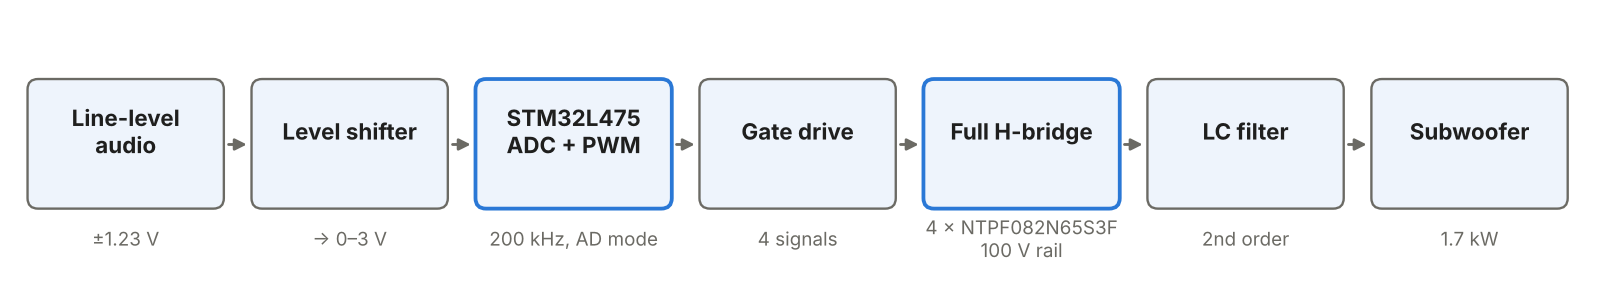
\includegraphics[width=\textwidth]{signal_chain.png}
\caption{Signal chain.}\label{fig:chain}
\end{figure}

\paragraph{Signal chain.} The line-level input ($\pm\SI{1.23}{\volt}$ from a jack) is shifted into the \SIrange{0}{3}{\volt} range of the microcontroller's ADC (Fig.~\ref{fig:chain}). The STM32L475 runs at \SI{80}{\mega\hertz} and compares each sample with a \SI{200}{\kilo\hertz} carrier to set the duty cycle. The bridge uses two-level (AD) modulation: leg~A has duty $d$ and leg~B has duty $1-d$, so the differential output is zero at $d=0.5$. Each leg needs a high-side and a low-side gate signal, separated by a dead time so that the two switches of a leg never conduct together. The power stage is a full H-bridge of four NTPF082N65S3F MOSFETs on a \SI{100}{\volt} rail, followed by a second-order LC filter.

\begin{table}[h]\centering\small
\begin{tabular}{lll}\toprule
Block & Part & Key parameters\\\midrule
Modulator & STM32L475VG (B-L475E-IOT01A) & Cortex-M4F, \SI{80}{\mega\hertz}, 12-bit ADC\\
Pre-amplifier (prototype) & TL081 op-amp & \SI{3.3}{\kilo\ohm}\,/\,\SI{1}{\kilo\ohm} gain network\\
Switches & NTPF082N65S3F ($\times4$) & \SI{650}{\volt}, $R_{DS(on)}\le\SI{82}{\milli\ohm}$, $Q_g=\SI{70}{\nano\coulomb}$, $Q_{rr}=\SI{397}{\nano\coulomb}$\\
Heatsink & CO2245V1 (one per device) & $R_{\theta SA}=\SI{7}{\celsius\per\watt}$, TO-220\\
Rail & DC supply & \SI{100}{\volt}\\\bottomrule
\end{tabular}
\caption{Main components.}\label{tab:parts}
\end{table}

\paragraph{Prototype.} The level shifter, pre-amplifier and gate-drive stages were built on breadboard (Fig.~\ref{fig:proto}). The H-bridge was built on a custom milled single-sided PCB with the four TO-220 devices and banana-jack power and output terminals. The full chain was assembled on the bench and reproduced audio through a small bookshelf loudspeaker at reduced rail voltage. In that test the loudspeaker's own inductance acted as the low-pass filter, because the LC filter was not populated.

\begin{figure}[t]\centering
\begin{subfigure}{0.27\textwidth}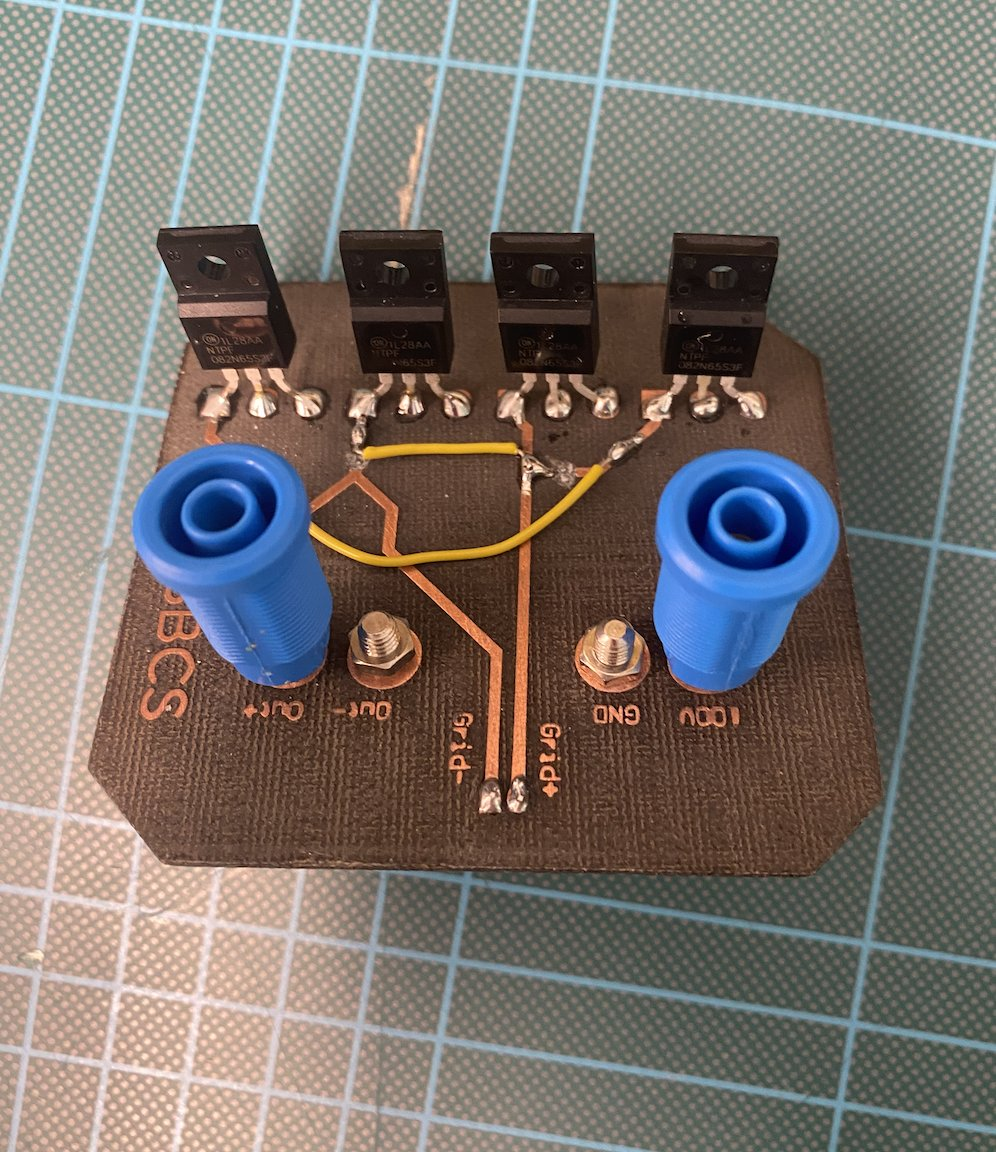
\includegraphics[width=\linewidth]{hbridge_pcb_top.jpg}\caption{H-bridge board.}\end{subfigure}\hfill
\begin{subfigure}{0.27\textwidth}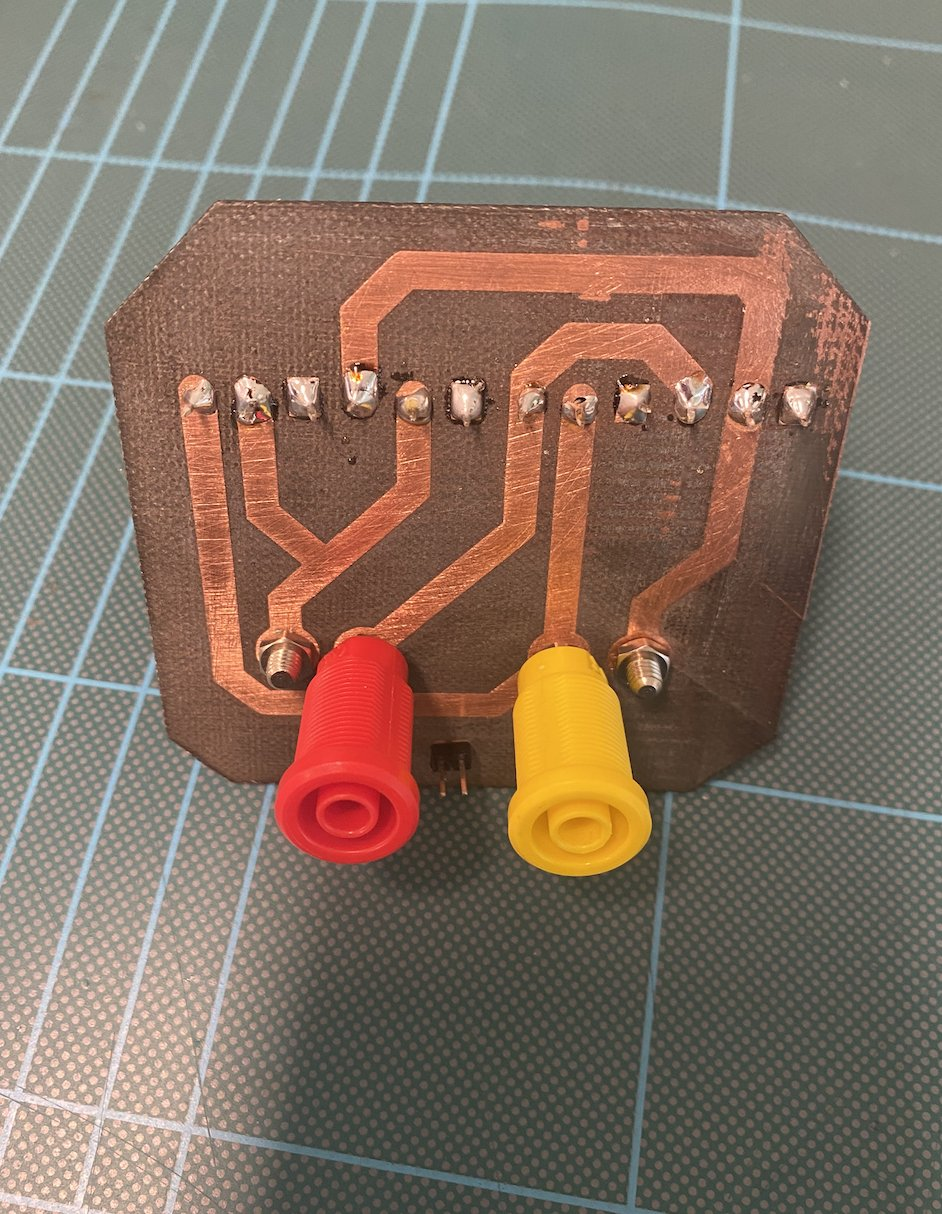
\includegraphics[width=\linewidth]{hbridge_pcb_bottom.jpg}\caption{Milled copper side.}\end{subfigure}\hfill
\begin{subfigure}{0.33\textwidth}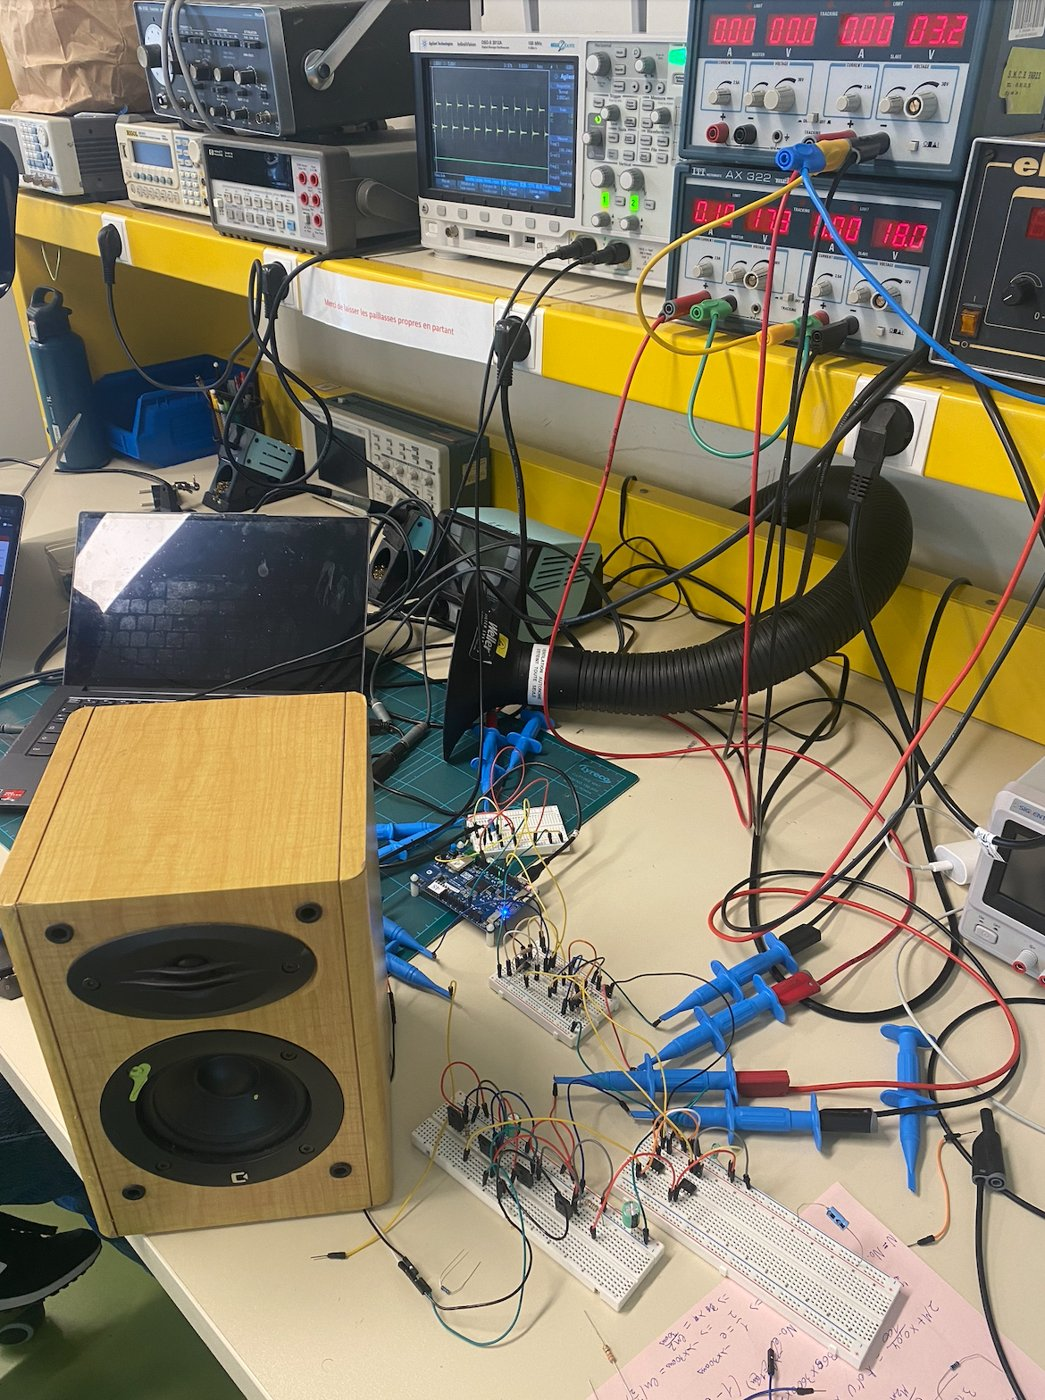
\includegraphics[width=\linewidth]{bench_setup.jpg}\caption{Bench audio test.}\end{subfigure}
\caption{Prototype hardware.}\label{fig:proto}
\end{figure}

\paragraph{Measured signals.} Fig.~\ref{fig:scope} shows three oscilloscope captures:
\begin{itemize}
\item \textbf{(a) Level shifter output:} the shifted audio sits inside the ADC range (\SI{1.73}{\volt} peak-to-peak with an \SI{82}{\hertz} test tone).
\item \textbf{(b) Microcontroller PWM output:} a \SI{3.3}{\volt}-logic square wave at \SI{195.8}{\kilo\hertz}, which is \SI{2}{\percent} below the \SI{200}{\kilo\hertz} nominal. The ringing on the edges is typical of a long probe ground lead.
\item \textbf{(c) Two antiphase signals at \SI{197.8}{\kilo\hertz}, \SI{7.0}{\volt} peak-to-peak:} their amplitude is above the \SI{3.3}{\volt} logic level and their shape is nearly sinusoidal. That identifies them as the outputs of the op-amp pre-amplifier, which is limited in bandwidth and slew rate. The node was inferred from the waveform and was not recorded at capture time. Section~\ref{sec:gate} explains why this stage cannot drive the MOSFETs at full rail.
\end{itemize}

\begin{figure}[t]\centering
\begin{subfigure}{0.32\textwidth}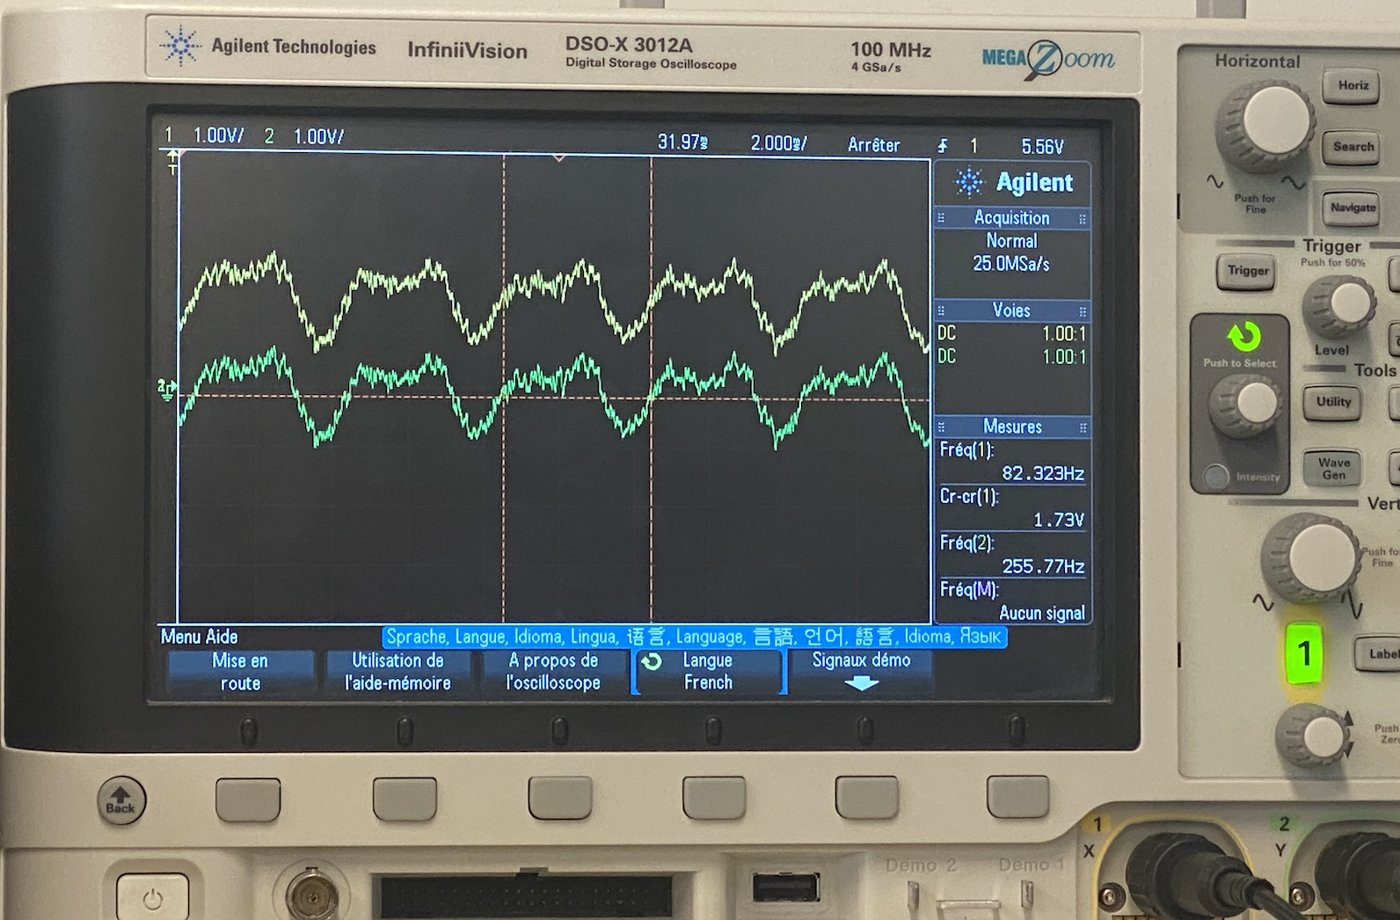
\includegraphics[width=\linewidth]{scope_level_shifter.jpg}\caption{Level-shifter output.}\end{subfigure}\hfill
\begin{subfigure}{0.32\textwidth}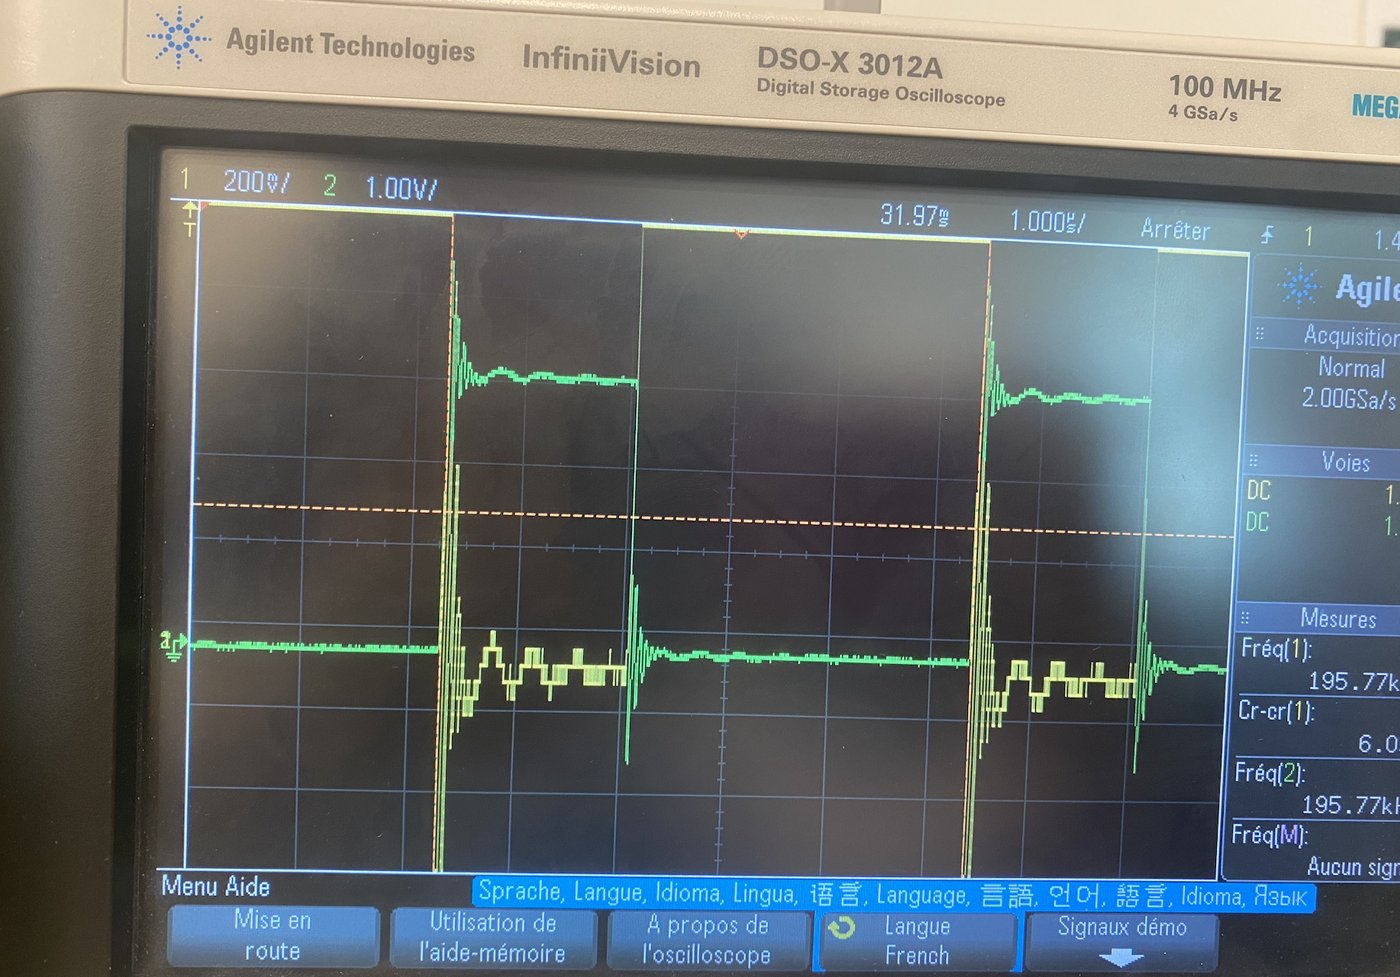
\includegraphics[width=\linewidth]{scope_switching_196kHz.jpg}\caption{MCU PWM, \SI{195.8}{\kilo\hertz}.}\end{subfigure}\hfill
\begin{subfigure}{0.32\textwidth}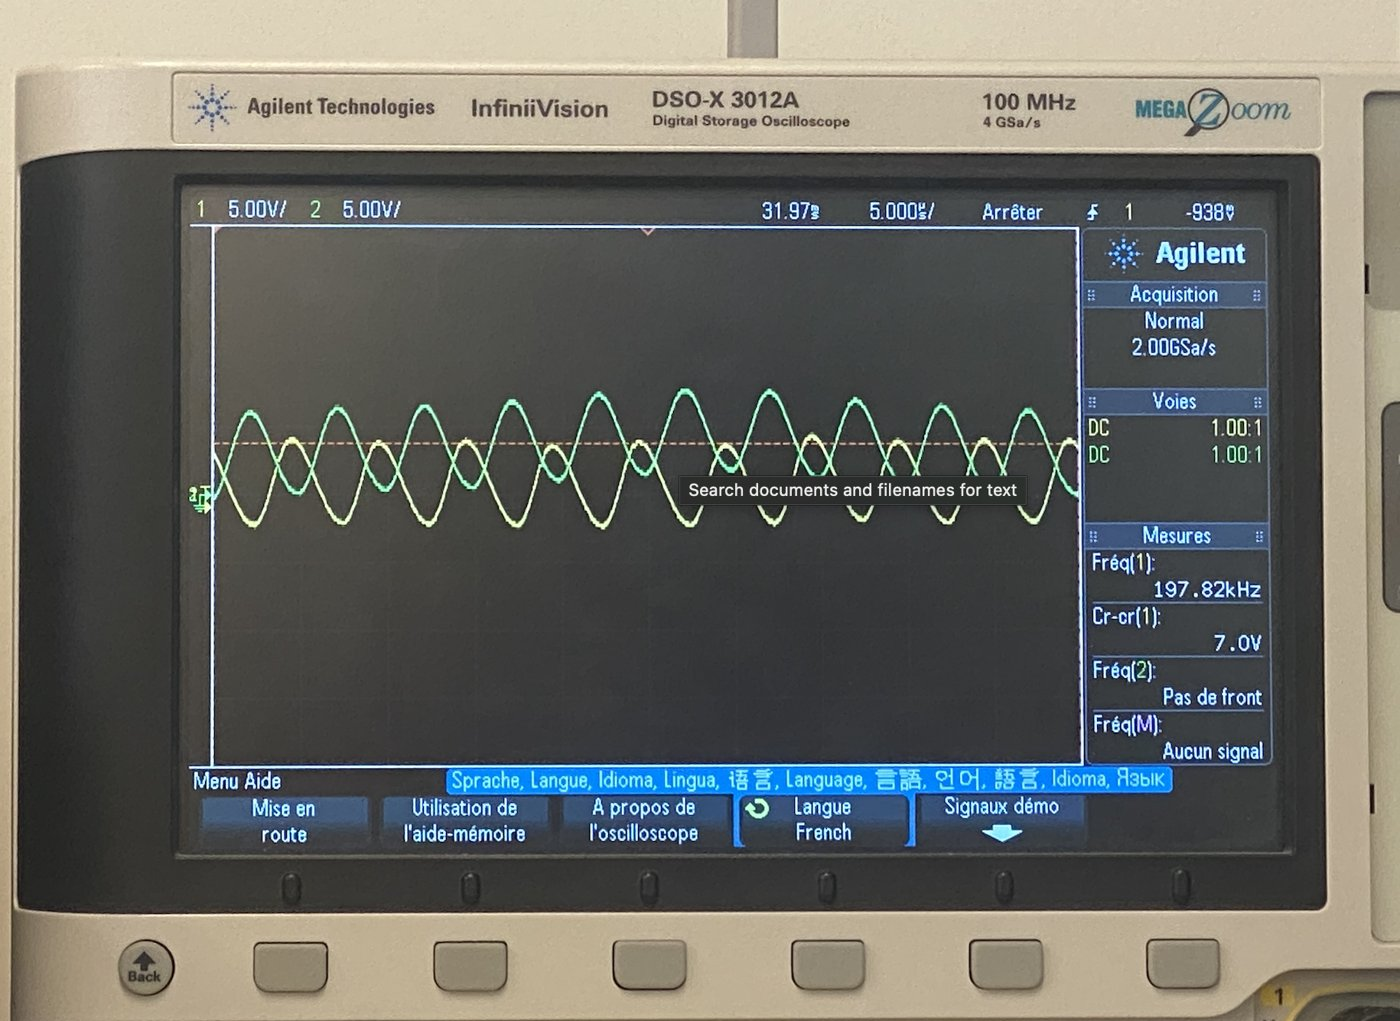
\includegraphics[width=\linewidth]{scope_preamp_197kHz.jpg}\caption{Pre-amplifier outputs.}\end{subfigure}
\caption{Measured signals (oscilloscope captures).}\label{fig:scope}
\end{figure}

\section{Design analysis}\label{sec:analysis}
The prototype ran at low voltage. This section uses datasheet values~\cite{onsemi} to determine what the \SI{100}{\volt}, \SI{1.7}{\kilo\watt} design requires. All numbers come from \texttt{analysis/power\_stage.py} and \texttt{analysis/pwm\_sim.py}.

\subsection{Deliverable power}
A full bridge at full modulation delivers an undistorted sine power of $P=V_\mathrm{bus}^2/2R$. On a \SI{100}{\volt} rail that is \SI{625}{\watt} into \SI{8}{\ohm}, \SI{1250}{\watt} into \SI{4}{\ohm} and \SI{2500}{\watt} into \SI{2}{\ohm}. The \SI{1.7}{\kilo\watt} target is therefore reachable only if the subwoofer's minimum impedance in band is at most \SI{2.94}{\ohm}. For an \SI{8}{\ohm} driver, the rail would have to rise to \SI{165}{\volt}. Measuring $|Z(f)|$ is the first step of the protocol (test~0).

\subsection{Losses, efficiency and thermal budget}
The model accounts for:
\begin{itemize}
\item conduction in the two devices carrying the load current, using $R_{DS(on)}=\SI{82}{\milli\ohm}\times1.5$ at $T_J=\SI{100}{\celsius}$ (datasheet Fig.~8);
\item V--I overlap at each hard transition;
\item body-diode reverse recovery;
\item $C_{oss}$ discharge ($E_{oss}=\SI{3.5}{\micro\joule}$ at \SI{100}{\volt});
\item diode conduction during the dead time.
\end{itemize}
The recovery charge is scaled with the commutated current; a constant \SI{397}{\nano\coulomb} gives a conservative bound.

\begin{table}[h]\centering\small
\begin{tabular}{lrrrrrr}\toprule
Operating point (\SI{2.94}{\ohm}) & Conduction & Overlap & Recovery & Other & Total & Per device\\\midrule
$\tfrac18$ power, \SI{212}{\watt} & 17.8 & 4.6 & 6.0 (15.6) & 2.6 & 30.9 (40.5) & 7.7 (10.1)\\
Full power, \SI{1.7}{\kilo\watt} & 142.2 & 13.0 & 16.8 & 4.7 & 176.8 & 44.2\\\bottomrule
\end{tabular}
\caption{Modelled stage losses in W. Values in parentheses use the constant-$Q_{rr}$ bound.}\label{tab:loss}
\end{table}

\begin{figure}[t]\centering
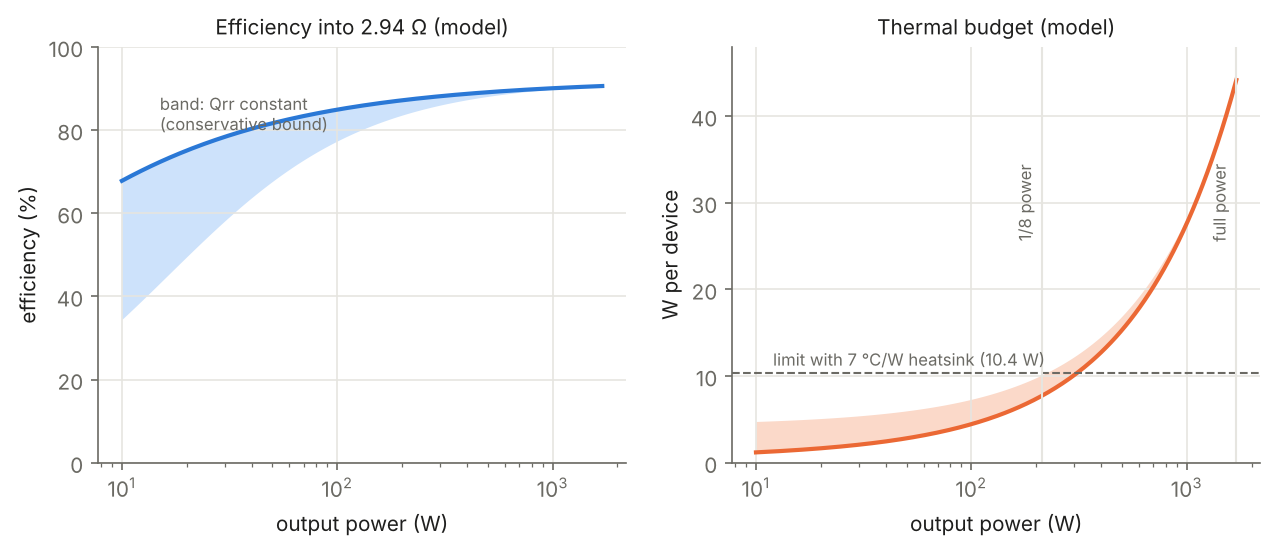
\includegraphics[width=\textwidth]{power_budget.png}
\caption{Modelled efficiency (left) and per-device dissipation (right) against output power into \SI{2.94}{\ohm}. The shaded band spans the two $Q_{rr}$ assumptions. Dashed line: the largest dissipation the \SI{7}{\celsius\per\watt} heatsink allows at \SI{45}{\celsius} ambient.}\label{fig:budget}
\end{figure}

The modelled efficiency at rated power is \SI{90.6}{\percent}, which meets the target. Conduction dominates (Table~\ref{tab:loss}). Thermally, each device may dissipate at most
\[
P_{\max}=\frac{T_{J,\max}-T_\mathrm{amb}}{R_{\theta JC}+R_{\theta CS}+R_{\theta SA}}=\frac{150-45}{2.62+0.5+7}=\SI{10.4}{\watt}.
\]
At $\tfrac18$ power, a common test condition for music signals, the model gives \SIrange{7.7}{10.1}{\watt} per device with $R_{DS(on)}$ taken at \SI{100}{\celsius}, so the selected heatsinks are marginal. Near \SI{150}{\celsius}, where the junction would actually sit, $R_{DS(on)}$ is higher still: with a factor of 1.9 to 2.2 the upper bound reaches \SIrange{11.3}{12.2}{\watt}, above the limit. The exact factor should be read from the datasheet before the heatsinks are chosen. At continuous full power, the \SI{44}{\watt} per device would raise the junction \SI{116}{\celsius} above the case through $R_{\theta JC}$ alone, which no heatsink can accommodate.

Sustained full power would therefore need lower conduction loss. A MOSFET rated for the actual \SI{100}{\volt} rail, rather than \SI{650}{\volt}, typically offers several times lower $R_{DS(on)}$ and recovery charge. Conduction loss scales linearly with $R_{DS(on)}$.

\subsection{Gate drive}\label{sec:gate}
Each MOSFET needs $Q_g=\SI{70}{\nano\coulomb}$ to switch. A general-purpose op-amp sources a few tens of milliamps, so charging the gate takes
\[
t \approx \frac{Q_g}{I}\approx\frac{\SI{70}{\nano\coulomb}}{\SI{20}{\milli\ampere}}=\SI{3.5}{\micro\second},
\]
which is longer than the \SI{2.5}{\micro\second} half-period at \SI{200}{\kilo\hertz}. The rounded \SI{7}{\volt} waveform in Fig.~\ref{fig:scope}c is consistent with this limit.

In addition, the two high-side N-channel devices need a gate voltage about \SI{10}{\volt} above their source, which sits at the rail when they conduct. A ground-referenced driver cannot provide that once the rail exceeds a few volts. A dedicated half-bridge gate driver with a bootstrap supply and an ampere-level peak current would switch the gate in tens of nanoseconds. It is the first change required before raising the rail.

\subsection{Output filter}
The schematic annotates each side of the filter with \SI{100}{\milli\henry} and \SI{470}{\nano\farad}. Into a \SI{4}{\ohm} load, these values give a corner at \SI{734}{\hertz}, but the series inductance attenuates the subwoofer band itself: \SI{-24}{\decibel} at \SI{50}{\hertz} (Fig.~\ref{fig:filter}). Such an inductor would also be impractically large at \SI{24}{\ampere} RMS. The values were most likely intended as \SI{100}{\micro\henry}, which gives a well-behaved low-pass filter.

A second-order Butterworth design for \SI{4}{\ohm} at \SI{20}{\kilo\hertz} uses \SI{22.5}{\micro\henry} and \SI{2.81}{\micro\farad} per side. It is flat over \SIrange{20}{200}{\hertz} and attenuates the carrier by \SI{40}{\decibel}.

\begin{figure}[t]\centering
\begin{minipage}{0.49\textwidth}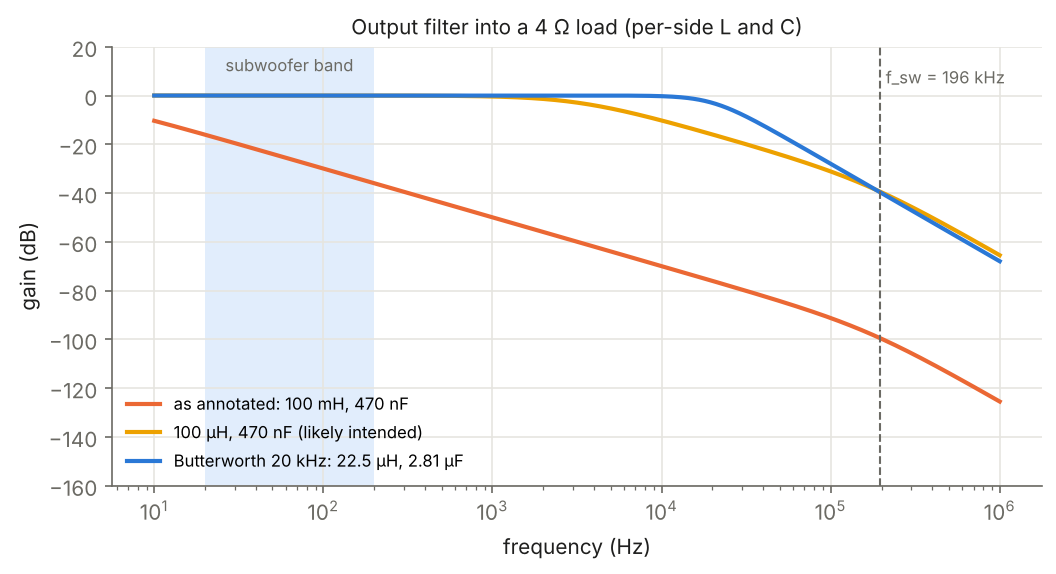
\includegraphics[width=\linewidth]{output_filter.png}\end{minipage}\hfill
\begin{minipage}{0.49\textwidth}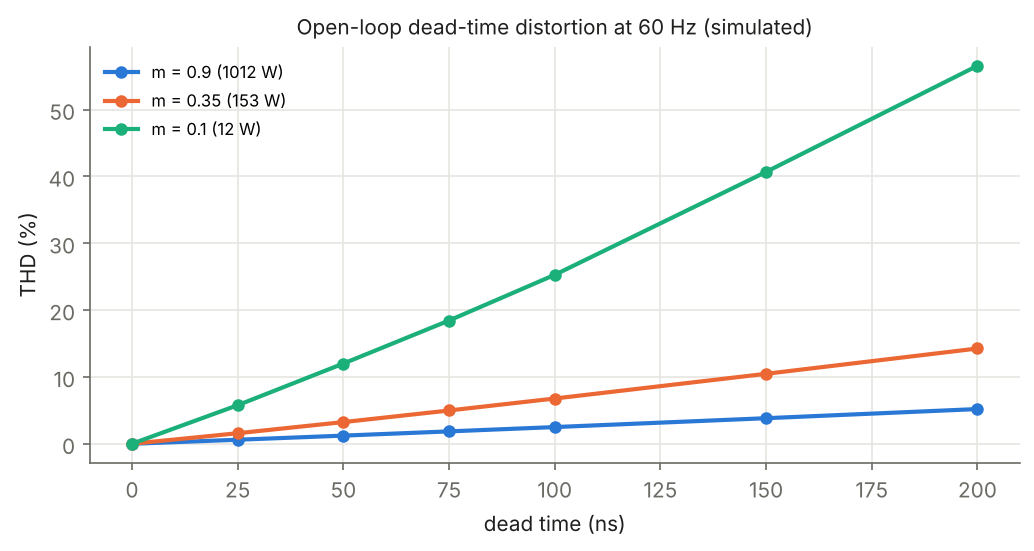
\includegraphics[width=\linewidth]{deadtime_thd.png}\end{minipage}
\caption{Left: transfer function of the output filter into \SI{4}{\ohm}. Right: simulated open-loop THD at \SI{60}{\hertz} against dead time, for three modulation depths.}\label{fig:filter}
\end{figure}

\subsection{Dead-time distortion and modulator resolution}
During each dead time, the leg voltage is set by the direction of the load current rather than by the modulator. Averaged over a switching period, this adds an error voltage of $2V_\mathrm{bus}f_\mathrm{sw}t_\mathrm{dead}\,\mathrm{sign}(i)$ across the load. At \SI{196}{\kilo\hertz} and \SI{150}{\nano\second}, that is \SI{5.9}{\percent} of the rail.

A cycle-averaged simulation through the Butterworth filter gives about \SI{10}{\percent} THD at \SI{153}{\watt} and much more at low level (Fig.~\ref{fig:filter}). The dead time therefore has to be as short as the MOSFET turn-off allows ($t_{d(off)}+t_f\approx\SI{70}{\nano\second}$ plus driver mismatch). Closed-loop feedback, which also improves PSRR, is the standard remedy. The original design plan already listed feedback as an improvement.

The PWM resolution is set by the timer: $f_\mathrm{clk}/f_\mathrm{sw}=400$ counts per period, or about \num{7.6} bits of duty-cycle resolution in centre-aligned mode. Section~\ref{sec:fw} recovers in-band resolution with noise shaping.

\section{Firmware redesign}\label{sec:fw}
The redesigned firmware (\texttt{firmware/}) is written against the CMSIS register definitions. It has four main features:

\paragraph{Gate timing.} TIM2 runs in centre-aligned mode at \SI{200}{\kilo\hertz}. Its four channels drive the four gates, using Arduino-header pins D1, D0, D10 and D4. High-side channels use PWM mode~1 and low-side channels use PWM mode~2. Their compare values sit $\pm6$ counts around the leg's switching point, which produces a \SI{150}{\nano\second} dead time on every edge without an advanced timer. The switching points are clamped so that every switch keeps a minimum on-time, which keeps a bootstrap supply charged.

\paragraph{Synchronised sampling.} The timer's update event triggers the ADC twice per PWM period (\SI{400}{\kilo S\per\second}). The conversion interrupt computes the next duty cycle, and preloaded compare registers apply it at the next update without glitches.

\paragraph{Signal processing.} A one-pole DC tracker (about \SI{1}{\hertz}) removes the level-shifter offset without calibration. First-order error-feedback noise shaping moves the quantisation error of the 7.6-bit compare value above the audio band. On the host, the in-band (\SIrange{20}{200}{\hertz}) SNR of the duty-cycle sequence for a \SI{60}{\hertz} tone rises from \SI{65.5}{\decibel} with plain rounding to \SI{98.2}{\decibel} with noise shaping. With an unquantised input it would reach \SI{127}{\decibel}: once the PWM is noise-shaped, the \SI{12}{bit} ADC sets the limit, and the real converter, whose effective resolution is below \SI{12}{bits}, will set it lower still.

\paragraph{Start-up.} The gate pins are held low as GPIO outputs. They are handed to the timer only after a \SI{500}{\milli\second} settling time, starting at \SI{50}{\percent} duty so that the load sees zero volts.

The firmware builds with \texttt{arm-none-eabi-gcc} to \SI{1.5}{\kilo\byte}. Host-side unit tests check the timing invariants on $10^6$ random inputs and the gain of a test tone; the dead time is checked on every sample. It has not yet been validated on hardware.

\section{Characterisation plan}\label{sec:protocol}
The targets are verified with the protocol in \texttt{docs/test-protocol.md}. It begins with a ramped power-up (\SIlist{12;24;48;100}{\volt}) on a non-inductive dummy load and takes measurements with a differential probe. The protocol has twelve tests:
\begin{itemize}
\item[0.] load impedance $|Z(f)|$;
\item[1.] switching signals, dead time and absence of shoot-through;
\item[2.] maximum power at \SI{1}{\percent} THD+N;
\item[3.] efficiency $\eta(P_\mathrm{out})$;
\item[4.] THD+N against power and frequency;
\item[5.] frequency response;
\item[6.] residual noise and dynamic range;
\item[7.] switching residual at the load;
\item[8.] PSRR;
\item[9.] DC offset and turn-on transient;
\item[10.] thermal steady state at $\tfrac18$ power;
\item[11.] a one-hour system test on the subwoofer.
\end{itemize}
Tests 3 and 4 are designed to calibrate the loss model and the dead-time simulation of Section~\ref{sec:analysis} against measurements. A helper script computes THD+N and output power from oscilloscope or sound-card captures.

\section{Conclusion and next steps}
The prototype demonstrated the complete chain, from audio input through microcontroller PWM to the H-bridge and audible output, at reduced voltage. The design analysis shows that the \SI{90}{\percent} efficiency target is plausible at rated power. It also shows that full power requires a load of at most \SI{2.94}{\ohm} and lower-$R_{DS(on)}$ devices for sustained operation.

The next steps, in order:
\begin{enumerate}
\item a bootstrap half-bridge gate driver;
\item protection before running at full rail voltage: a stalled or halted firmware freezes the duty cycle and can put DC across the subwoofer, so the design needs DC-offset detection with an output relay, a watchdog, and overcurrent shutdown (TIM1 and TIM8 have a hardware break input; TIM2 does not);
\item MOSFETs rated for the \SI{100}{\volt} rail rather than \SI{650}{\volt};
\item a correctly dimensioned LC filter;
\item a two-layer PCB with a tight switching loop to reduce the ringing seen in Fig.~\ref{fig:scope}b;
\item closed-loop feedback to suppress dead-time distortion and supply ripple;
\item the characterisation protocol of Section~\ref{sec:protocol}.
\end{enumerate}

\begin{thebibliography}{9}\small
\bibitem{onsemi} onsemi. \textit{NTPF082N65S3F Power MOSFET, N-Channel, SUPERFET III FRFET, 650 V, 40 A, 82 m$\Omega$}. Datasheet rev.~4, 2018.
\bibitem{infineon} Infineon Technologies. \textit{Class D Audio Amplifier Design}. Training material, v01\_00.
\bibitem{aes17} Audio Engineering Society. \textit{AES17-2020: AES standard method for digital audio engineering -- Measurement of digital audio equipment}.
\end{thebibliography}
\end{document}
